% Created 2020-05-15 Fri 17:08
% Intended LaTeX compiler: pdflatex
\documentclass[presentation]{beamer}
\usepackage[utf8]{inputenc}
\usepackage[T1]{fontenc}
\usepackage{graphicx}
\usepackage{grffile}
\usepackage{longtable}
\usepackage{wrapfig}
\usepackage{rotating}
\usepackage[normalem]{ulem}
\usepackage{amsmath}
\usepackage{textcomp}
\usepackage{amssymb}
\usepackage{capt-of}
\usepackage{hyperref}
\usetheme{UoB}
\author{Mark Blyth}
\date{}
\title{GPR on non-trivial data}
\hypersetup{
 pdfauthor={Mark Blyth},
 pdftitle={GPR on non-trivial data},
 pdfkeywords={},
 pdfsubject={},
 pdfcreator={Emacs 26.3 (Org mode 9.1.9)}, 
 pdflang={English}}
\begin{document}

\maketitle

\section{Background}
\label{sec:org56b3de2}
\begin{frame}[label={sec:org8056e5e}]{Week's work}
\begin{itemize}
\item Redraft the continuations paper
\begin{itemize}
\item Done, but I want another full read
\end{itemize}
\item Test GPR on various different cases
\begin{itemize}
\item Different models
\item Stochastic and deterministic simulations
\item Many and few datapoints
\end{itemize}
\item Other stuff: tidied up my assortments of codes
\end{itemize}
\end{frame}

\section{Models}
\label{sec:org87f1c14}
\begin{frame}[label={sec:orgab5deeb}]{Stochasticity}
\begin{itemize}
\item Looked into stochastic neuron models
\begin{itemize}
\item They're hard -- requires stochastic calculus, stochastic integrators, etc., which I don't know anything about
\end{itemize}
\item Produce all sorts of non-trivial dynamics
\begin{itemize}
\item Stochastic and coherence resonance
\item P-bifurcations
\end{itemize}
\end{itemize}

\vfill

\begin{itemize}
\item Very interesting area, but also another can of worms
\item Suggestion: test GPR on deterministic models + noise, then move on to stochastics
\begin{itemize}
\item Start reading a stochastics textbook?
\end{itemize}
\end{itemize}
\end{frame}

\begin{frame}[label={sec:orge4e8875}]{GPR testing}
\begin{itemize}
\item Set up a script to generate lots of neuron simulations \emph{[next slides]}
\item Working on adding in the simpler kernels I've been playing with
\item Goal: test\ldots{}
\begin{itemize}
\item four models (FH, HR, HR fast, HH)\ldots{}
\item with three kernels (SE, modulo, cosine)\ldots{}
\item with and without noise
\end{itemize}
\item 24 different cases
\begin{itemize}
\item The code structure makes it easy to switch between cases
\item Taking a long time to fit each kernel (log-likelihood had an error!)
\end{itemize}
\end{itemize}
\end{frame}

\begin{frame}[plain,label={sec:org28022af}]{Neuron models - Fitzhugh Nagumo}
\begin{center}
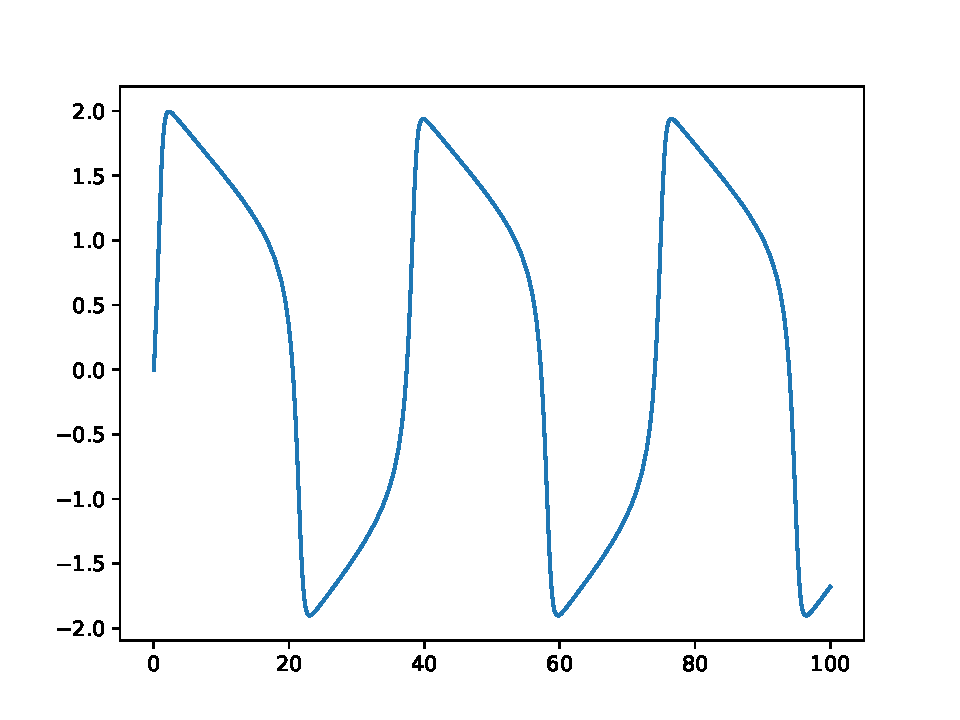
\includegraphics[width=\textwidth]{./clean_FH.pdf}
\end{center}
\end{frame}

\begin{frame}[plain,label={sec:org618809b}]{Fitzhugh Nagumo, SEKernel}
\begin{center}
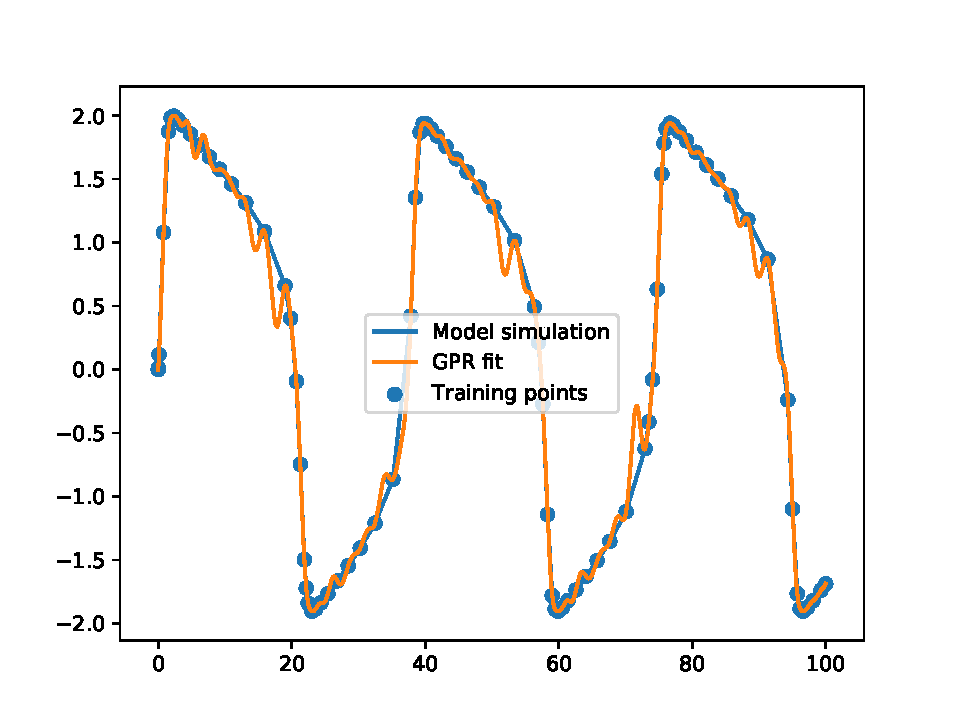
\includegraphics[width=\textwidth]{./FH_SEKernel.pdf}
\end{center}
\end{frame}

\begin{frame}[plain,label={sec:orge16959a}]{Fitzhugh Nagumo, modulo kernel}
\begin{center}
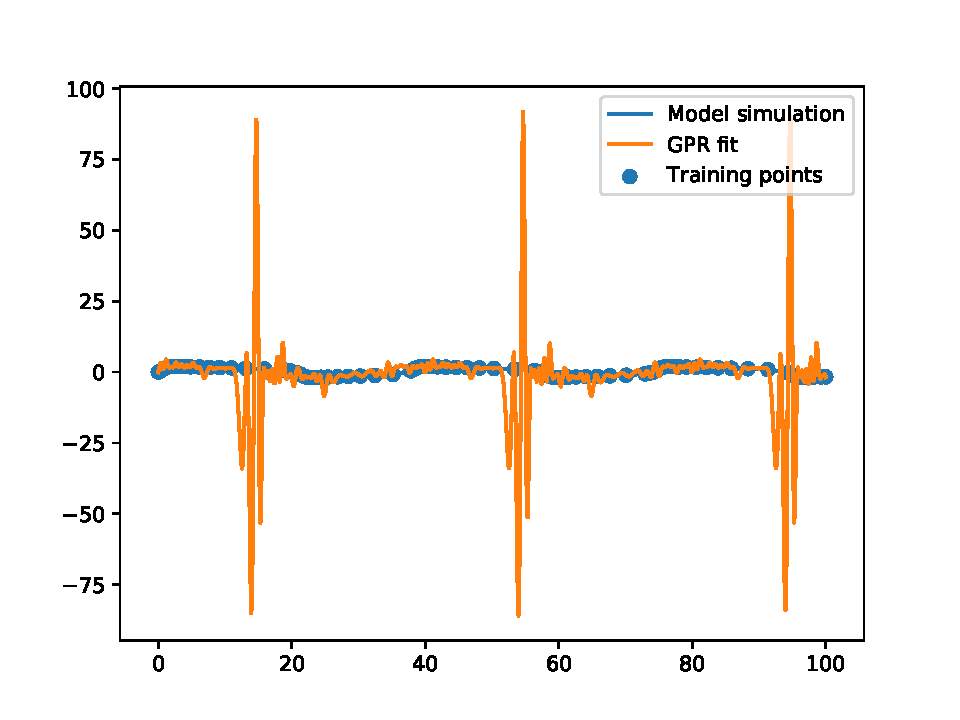
\includegraphics[width=\textwidth]{./FH_Modulo.pdf}
\end{center}
\end{frame}

\begin{frame}[plain,label={sec:orgff5d456}]{Fitzhugh Nagumo, cosine kernel}
\begin{center}
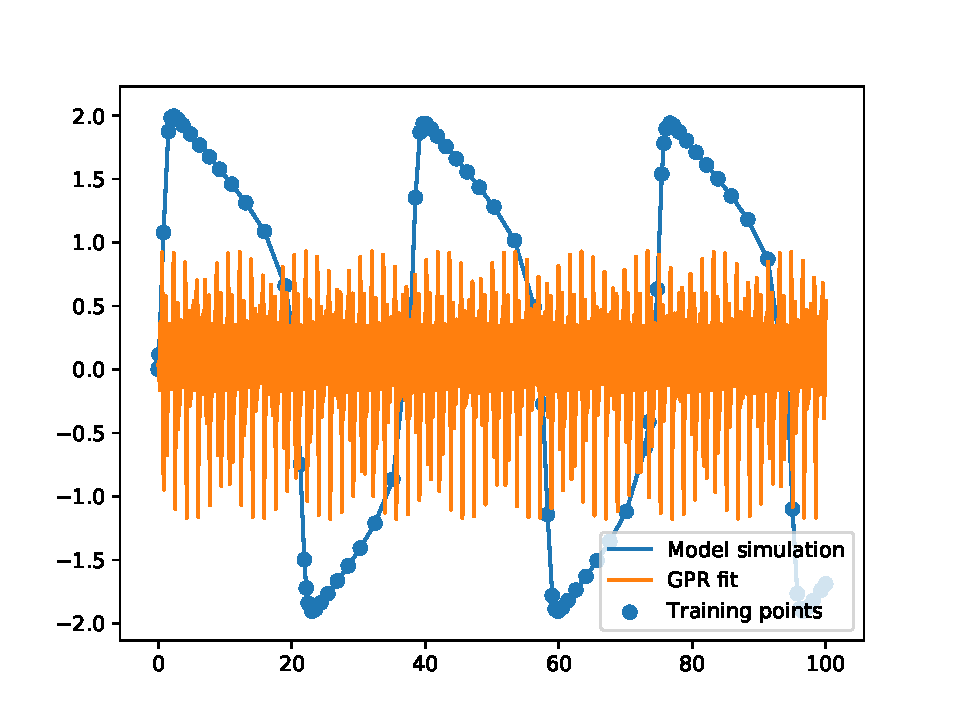
\includegraphics[width=\textwidth]{./FH_CosineKernel.pdf}
\end{center}
\end{frame}

\begin{frame}[plain,label={sec:org6a9043a}]{Neuron models - Hindmarsh Rose fast subsystem}
\begin{center}
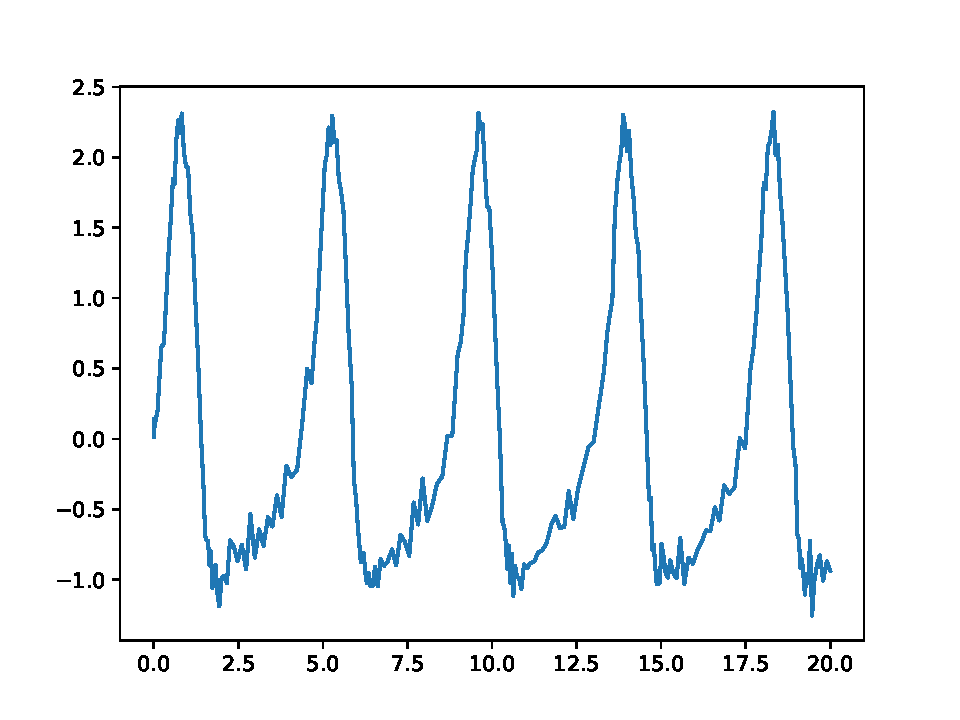
\includegraphics[width=\textwidth]{./noisy_HR_fast.pdf}
\end{center}
\end{frame}

\begin{frame}[plain,label={sec:org67a6722}]{Neuron models - Hodgkin Huxley}
\begin{center}
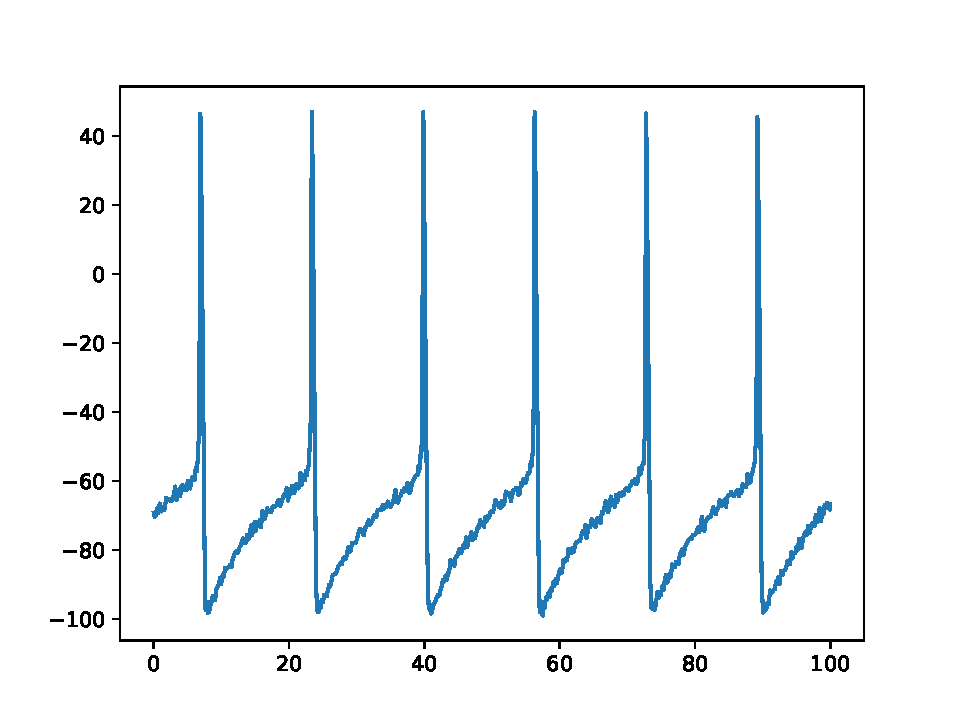
\includegraphics[width=\textwidth]{./noisy_HH.pdf}
\end{center}

(This took a long time!)
\end{frame}

\begin{frame}[plain,label={sec:orgc73c4d1}]{Hodgkin Huxley SEKernel}
\begin{center}
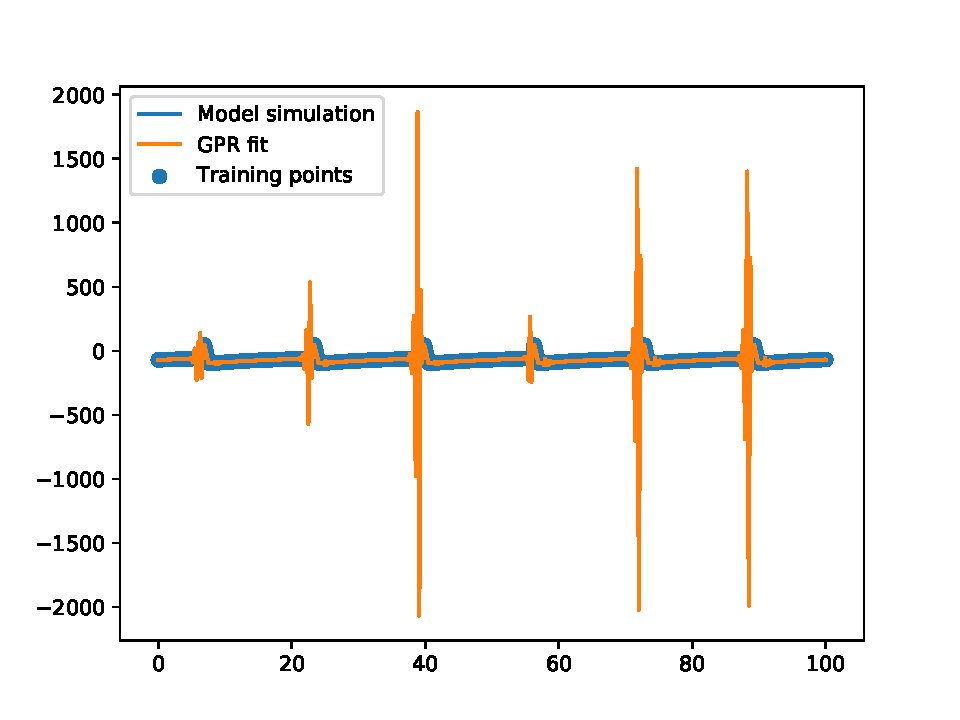
\includegraphics[width=\textwidth]{./HH_SEKernel.pdf}
\end{center}
\end{frame}

\begin{frame}[plain,label={sec:orge2a730d}]{Hodgkin Huxley SEKernel}
\begin{center}
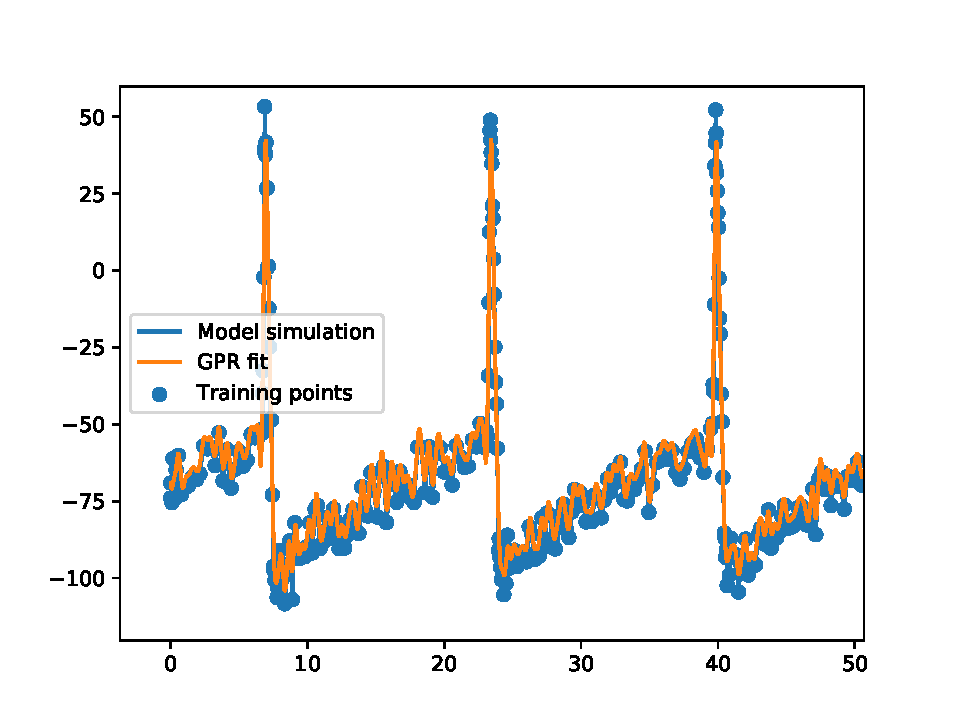
\includegraphics[width=\textwidth]{./HH_noise.pdf}
\end{center}
\end{frame}

\begin{frame}[plain,label={sec:org289d05f}]{Neuron models}
\begin{center}
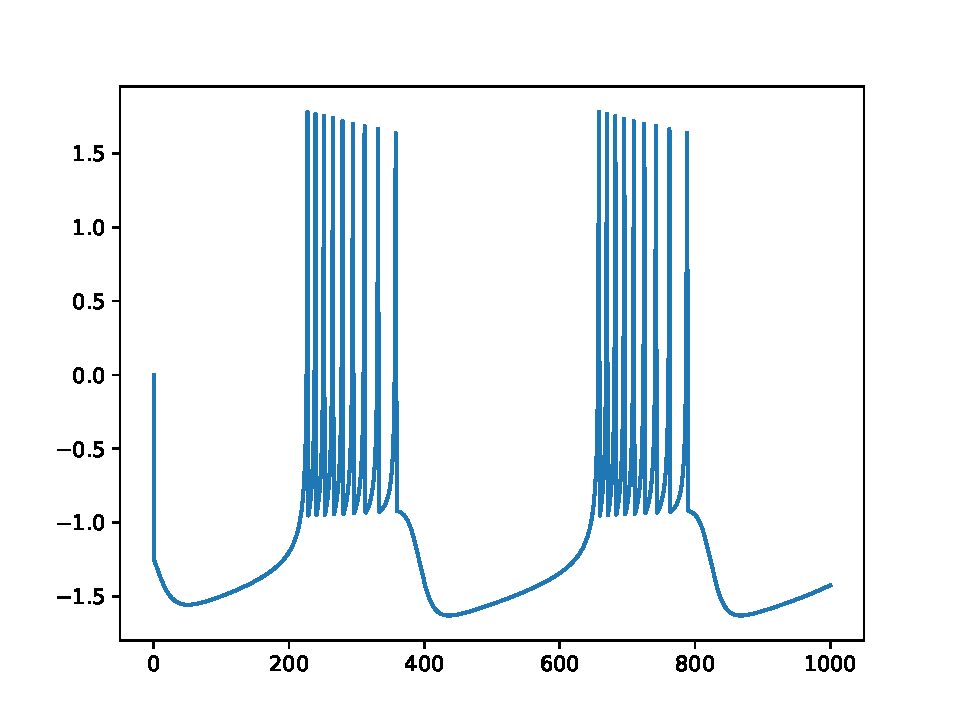
\includegraphics[width=\textwidth]{./clean_HR.pdf}
\end{center}
\end{frame}

\section{Next steps}
\label{sec:org522a746}
\begin{frame}[label={sec:orgfd2a10e}]{Codes}
CBC code:

\url{https://github.com/MarkBlyth/SingleCellCBC}

\vfill
GPR code:

\url{https://github.com/MarkBlyth/gpr\_tests}

\vfill

Can also put presentations on GitHub?
\end{frame}

\begin{frame}[label={sec:orgb1c507c}]{Next steps}
\begin{itemize}
\item \emph{[More]} teaching
\item Full re-read of paper
\end{itemize}
\vfill

then\ldots{}

\vfill
\begin{itemize}
\item More GPR testing
\begin{itemize}
\item Add more kernels into the testing setup
\item Test everything!
\end{itemize}
\end{itemize}
\end{frame}
\end{document}
